\documentclass{article}
\usepackage{graphicx}
\usepackage{caption}
\graphicspath{ {./images/} }
 
\begin{document}
\paragraph{A first Look at the Captured Trace}
  \begin{enumerate}
    \item What is the IP Address and TCP port number used by the client computer that is transferring the file to gaia.cs.umass.edu?
      \begin{itemize}
        \item IP Address: 10.106.0.254
        \item TCP Port Number: 55011
        \item 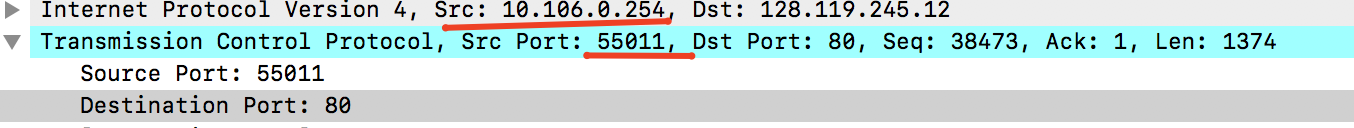
\includegraphics[scale=0.5]{images/TCP1.png}
      \end{itemize}
    \item What is the IP address of gaia.cs.umass.edu?  On what port number is it sending and receiving TCP segments for this connection?
        \begin{itemize}
          \item IP Address: 128.119.245.12
          \item TCP Port Number: 80
          \item 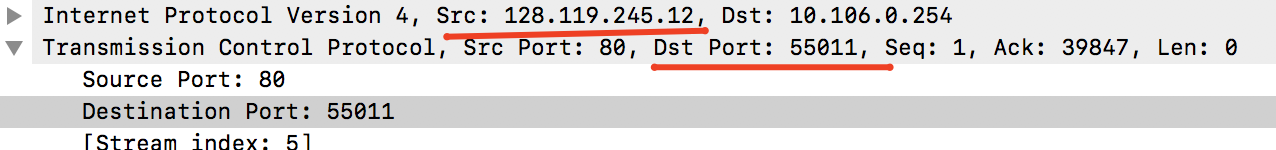
\includegraphics[scale=0.5]{images/TCP2.png}
        \end{itemize}

    \item What is the IP address and TCP port number used by your client computer to transfer the file to gaia.cs.umass.edu?
        \begin{itemize}
        \item IP Address: 10.106.0.254
        \item TCP Port Number: 55011
        \end{itemize}

    \item What is th sequence number of the TCP SYN segment that is used to initiate the TCP connection between the client computer and gaia.cs.umass.edu?
    What is it in the segment that identifies the segment as a SYN segment?
        \begin{itemize}
          \item Sequnce Number: 0
          \item The segment is identified as a SYN segment because in the flags field the SYN bit is set to 1.
          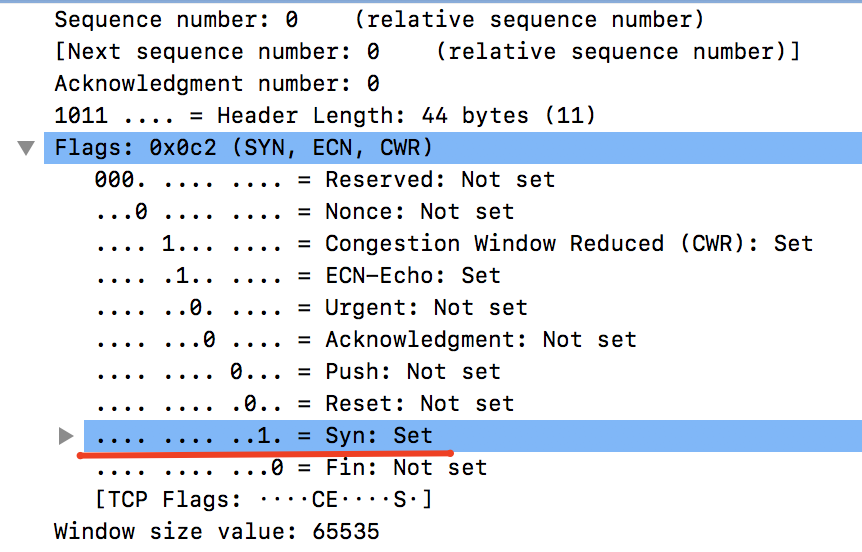
\includegraphics[scale=0.5]{images/TCP4.png}
        \end{itemize}

    \paragraph{TCP Basics}
    \item What is the sequence number of the SYNACK segment seny by gaia.cs.umass.edu to the client computer in reply to the SYN?  What ist he value of the Acknowledgment field in the SYNACK segment?  How did 
    gaia.cs.umass.edu determine that value?  What is it in the segment that identifies the segment as a SYNACK segment?
        \begin{itemize}
          \item Sequence Number: 0
          \item Acknowledgement Field: 1
          \item It is calculated by taking the sequence number from the SYN added with its length in bytes.
          \item The segment is identified by its field value, similaraly to the SYN segment, the SYN and Acknowledgement bits are set.
          \item 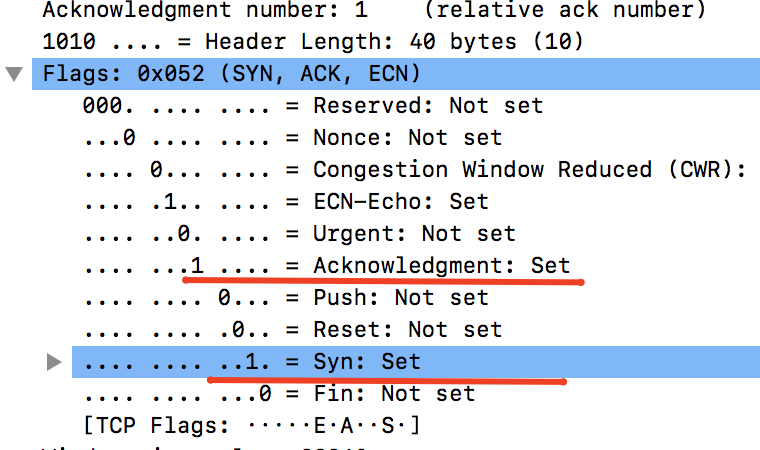
\includegraphics[scale=0.5]{images/TCP5.png}
        \end{itemize}

    \item What is the sequence number of the TCP segment containing the HTTP POST command?  Note that in order to find the POST command, you'll need to dig into the packet content field at the bottom 
    of the wireshark window, looking for a segment with a "POST" within its DATA field
        \begin{itemize}
          \item Sequence Number: 1
          \item 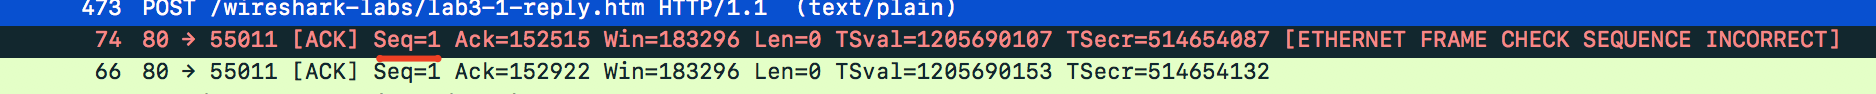
\includegraphics[scale=0.5]{images/TCP6.png}
        \end{itemize}

    \item Consider the TCP segment containing the HTTP POSt as the first segment in the TCP connection.  What are the sequence numbers of th first six segments in th TCP connection?  At what time was each segment sent?  When was the ACK for each segment received?  Given the difference between when each TCP segment was seent, and when its acknowledgment was received, what is the RTT value for eeaech of the six segments?  What is the EstimatedRTT value after the receipt of each ACK?  Assume that the value of the Estimated RTT is equal to th measured RTT for the first segment, and then is computed using the EstimatedRTT equation
        \begin{itemize}
          \item 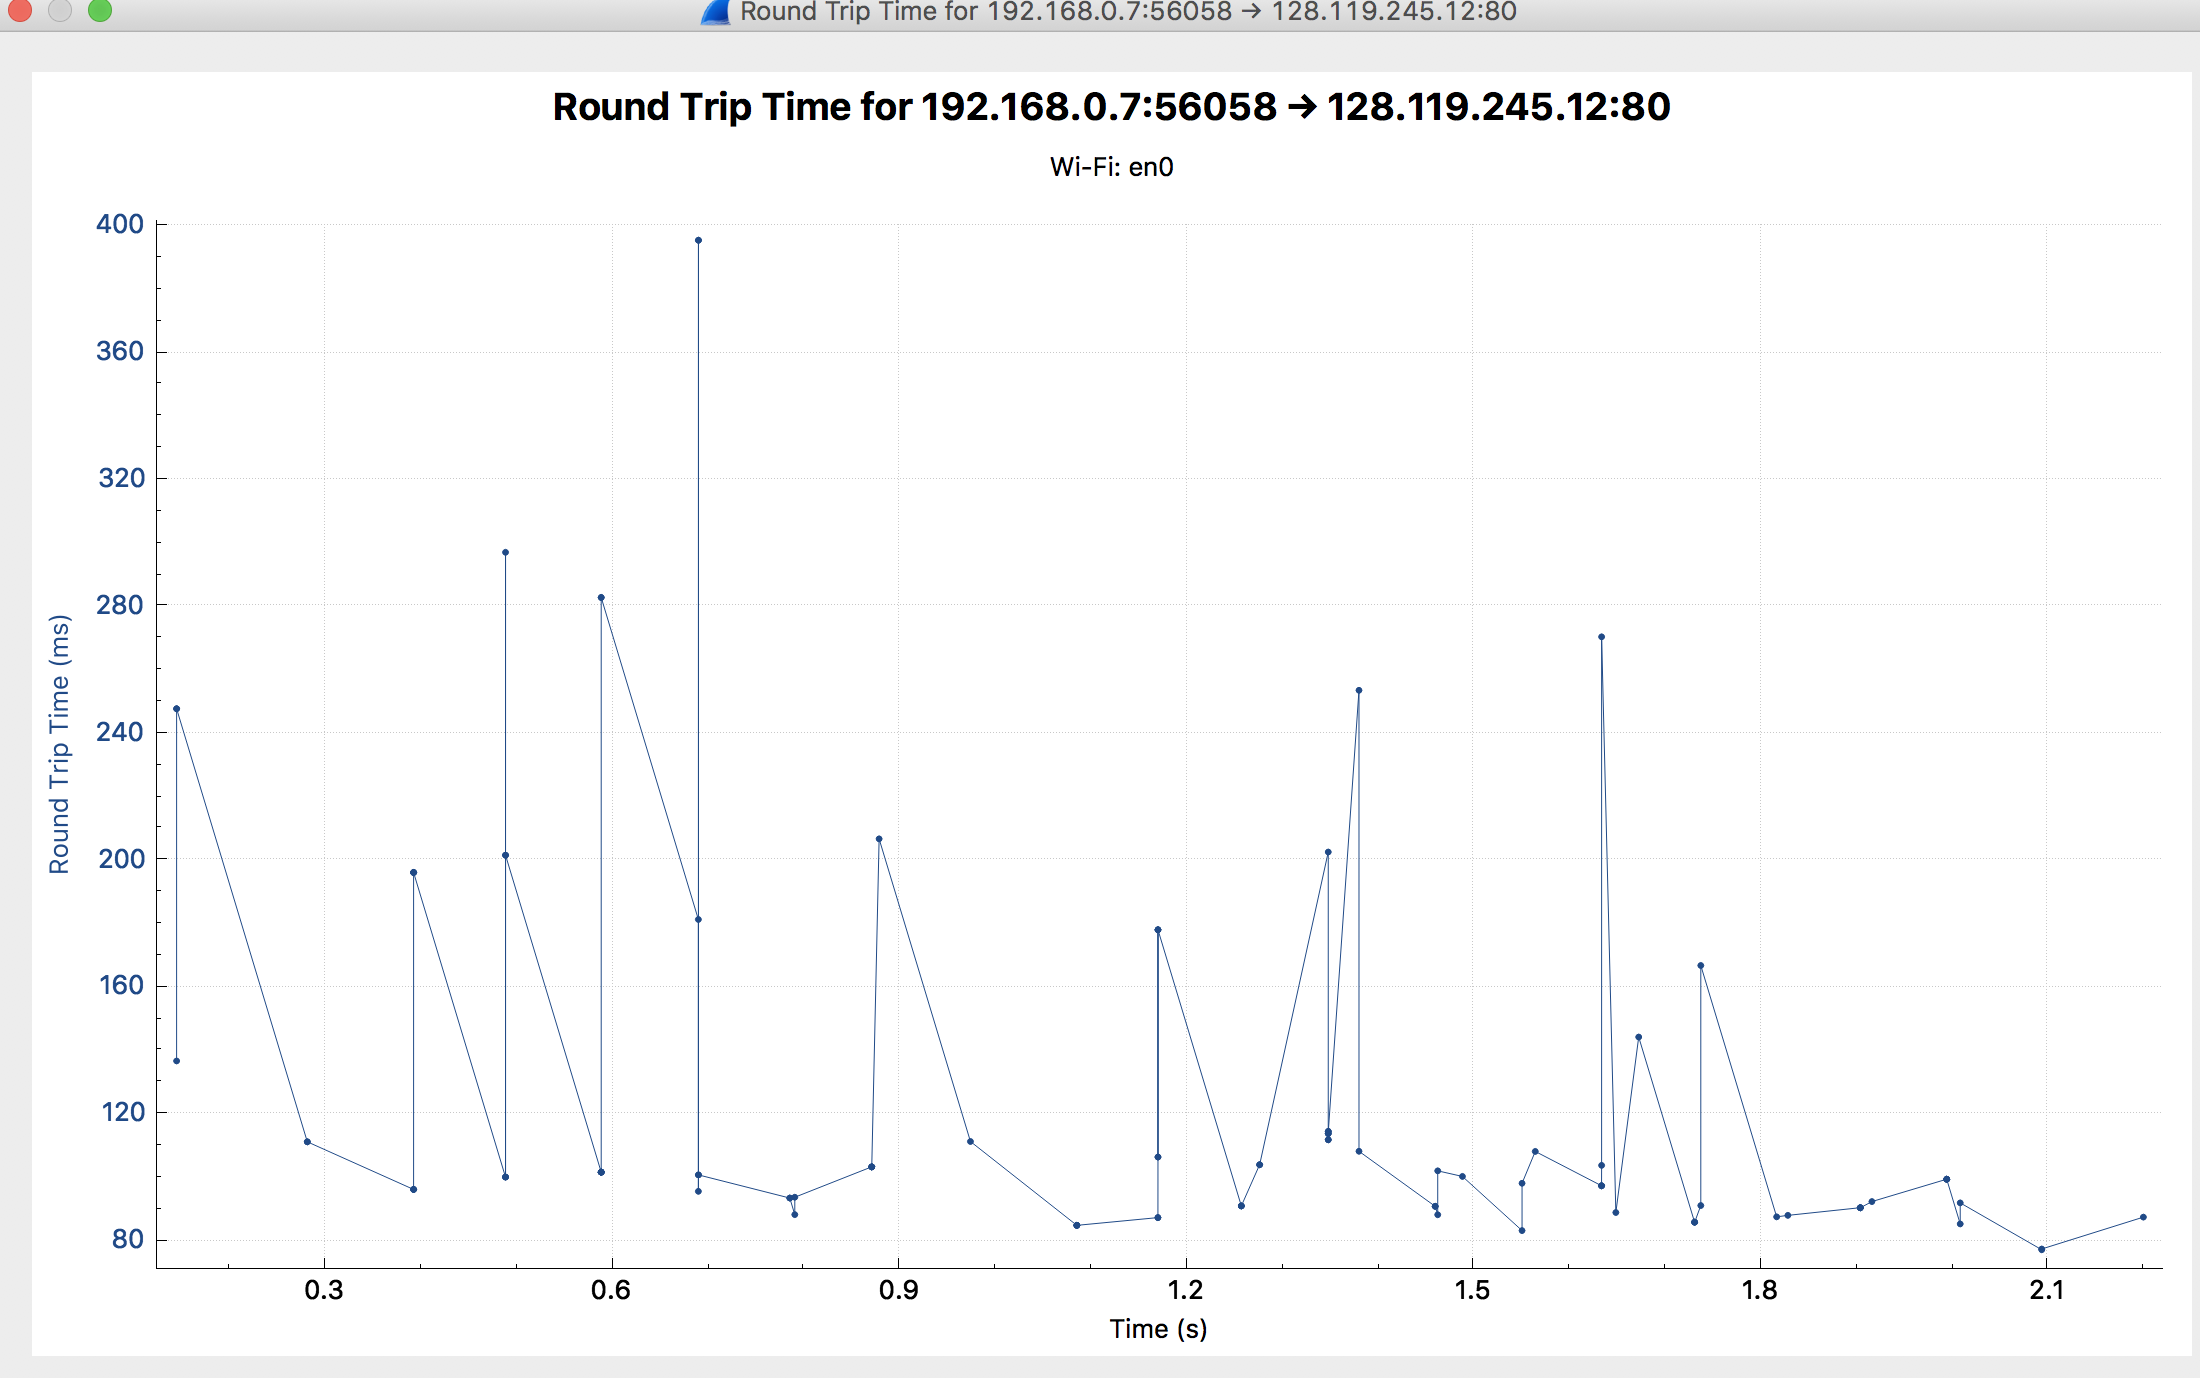
\includegraphics[scale=0.3]{images/TCPRTT.png}
        \end{itemize}
    \item What is the length of each of the first TCP segments?
        \begin{itemize}
          \item The length of the TCP segment with the POST request is 881 bytes
          \item 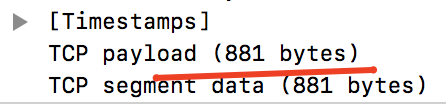
\includegraphics[scale=0.5]{images/TCPPOST.png}
          \item The length of the remaining TCP segments is 1448 bytes
          \item 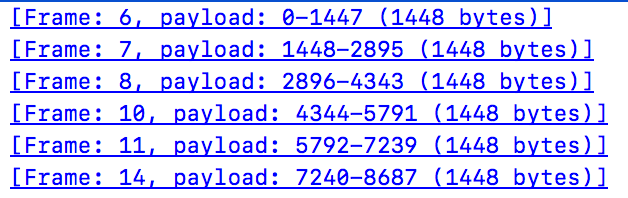
\includegraphics[scale=0.5]{images/TCPSG.png}
        \end{itemize}

    \item What is the minimum amount of available buffer space advertised at the recived for the entire trace?  Does the lack of receiver buffer space ever throttle the sender?
        \begin{itemize}
          \item The minimum amount of available buffer space is 1431 * (128) bytes
          \item The lack of receiver buffer space does not throttle the sender
          \item 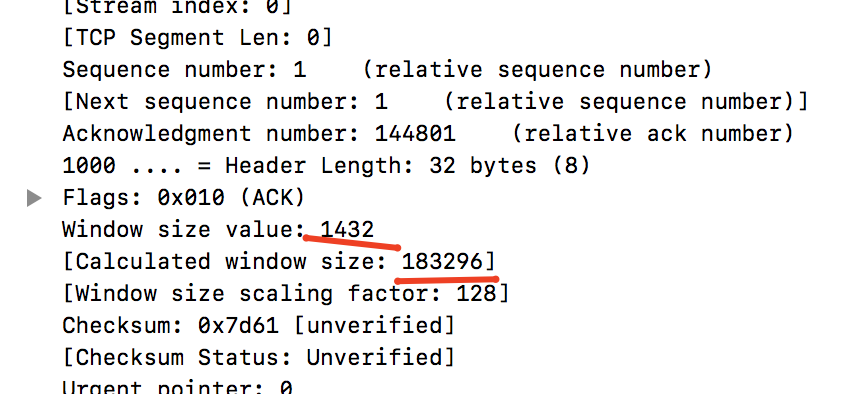
\includegraphics[scale=0.5]{images/TCPWIN.png}
        \end{itemize}

    \item Are there any retransmitted segments in the trace file?  What did oyu check for (in the trace) in order to answer this question?
        \begin{itemize}
          \item 
        \end{itemize}

    \item How much data does ther eceiver typically Acknowlede in an ACK?  Can you identify cases where the receiver is ACKing every other recived segment?
        \begin{itemize}
          \item 
        \end{itemize}

    \item What is the throughput for the TCP connection?
        \begin{itemize}
          \item The throughput is 800k bits/s
          \item 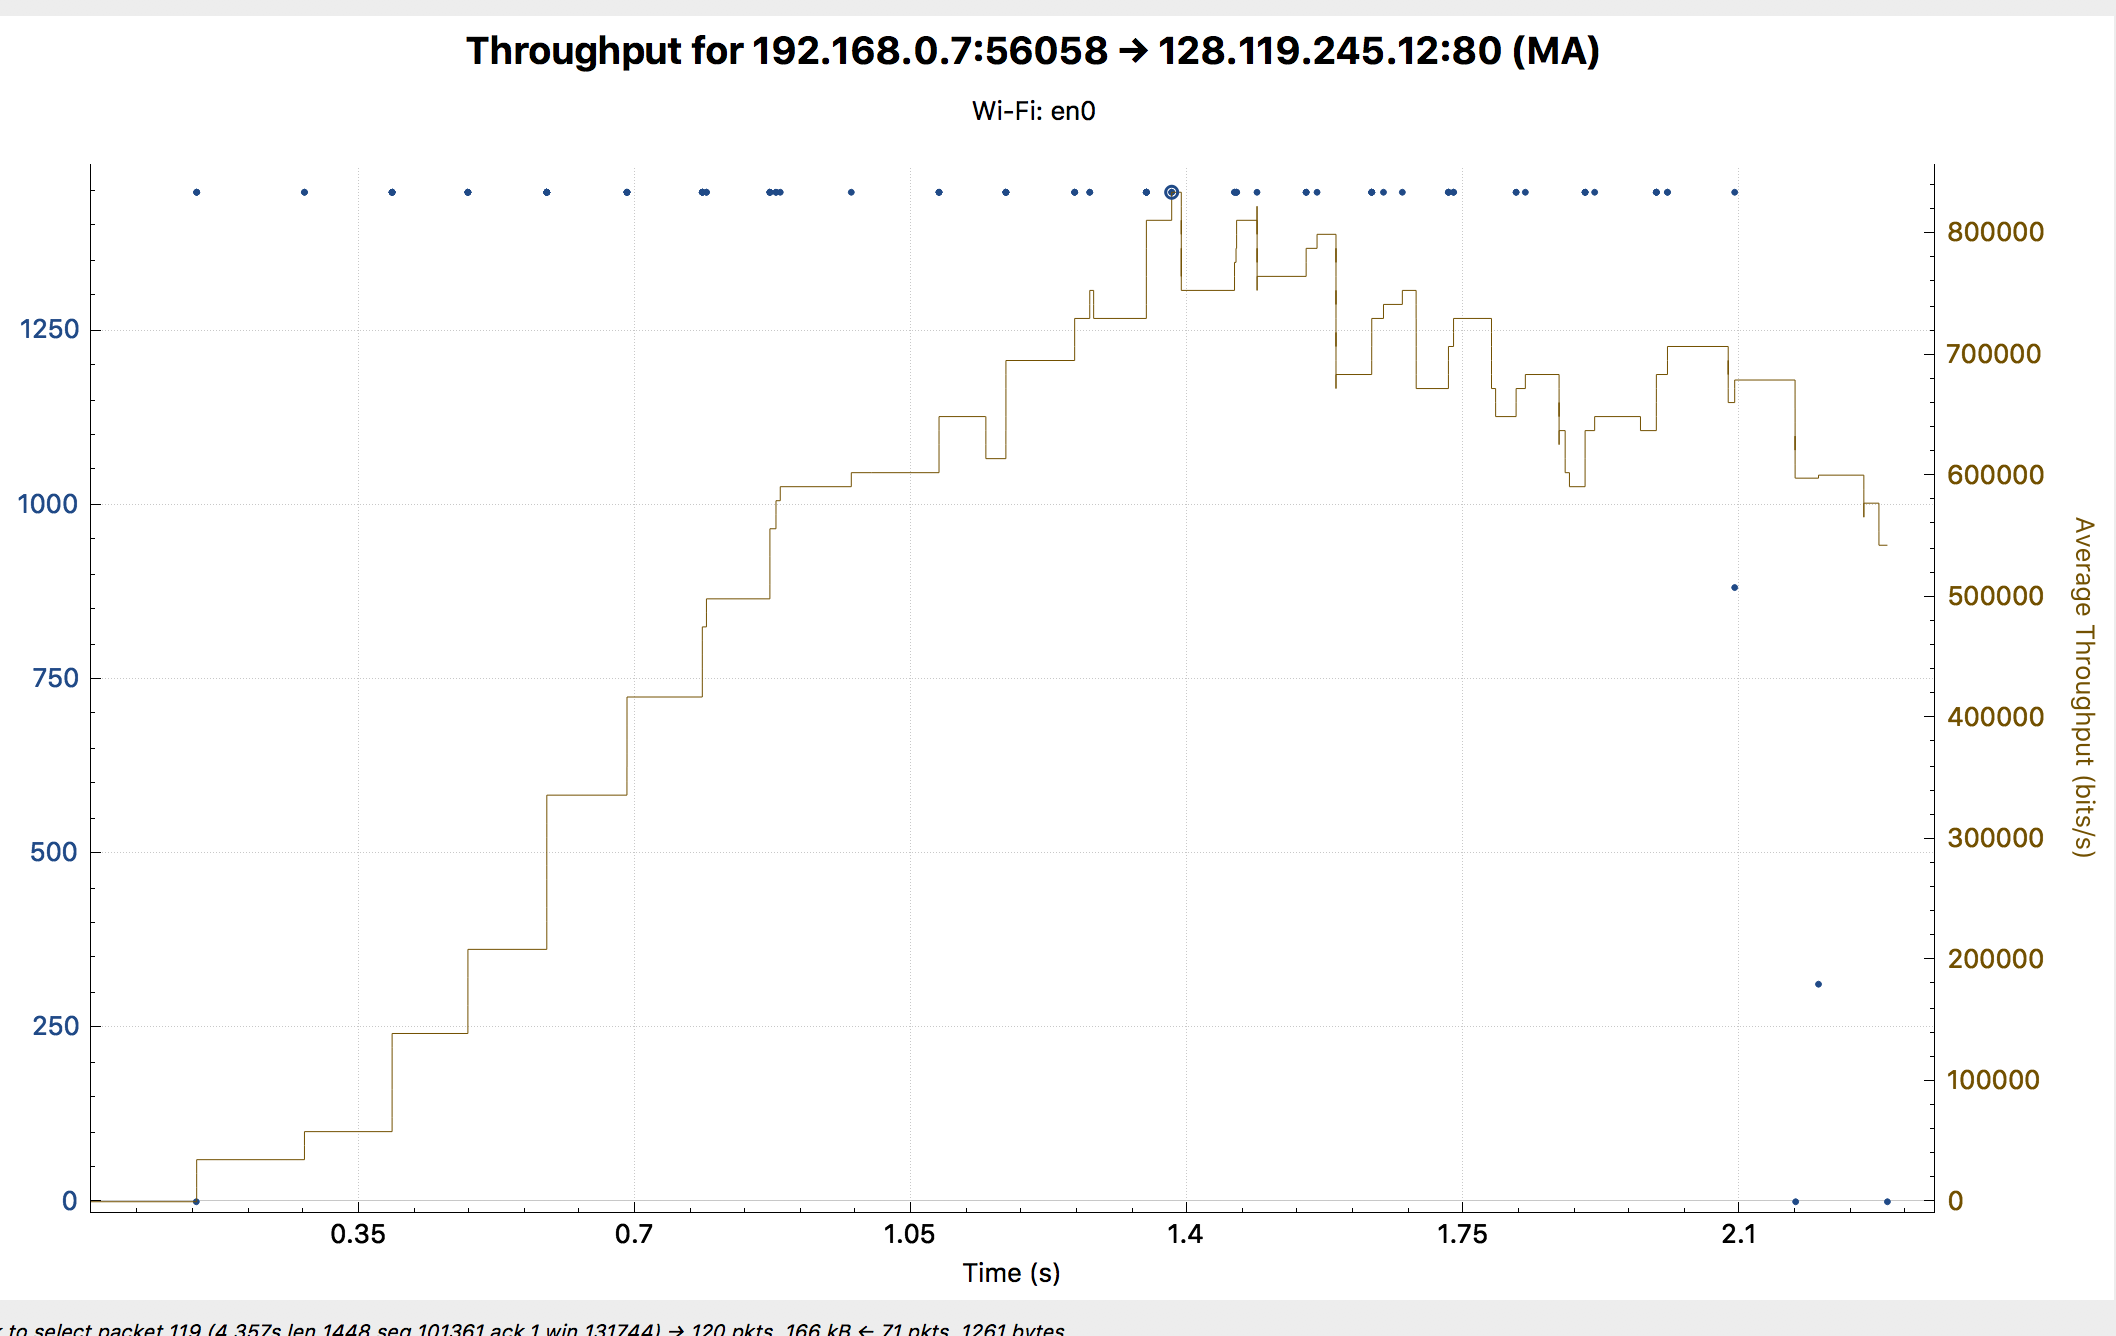
\includegraphics[scale=0.3]{throughput.png}
        \end{itemize}
    \paragraph{TCP congestion control in action}
    \item Can you identify where TCP's slowstart phase begins and ends, and where congestiong avoidance takes over?  Commen onw ays in which the measured data differs from the idealized behavior of TCP that we've
    studied in the text
        \begin{itemize}
          \item 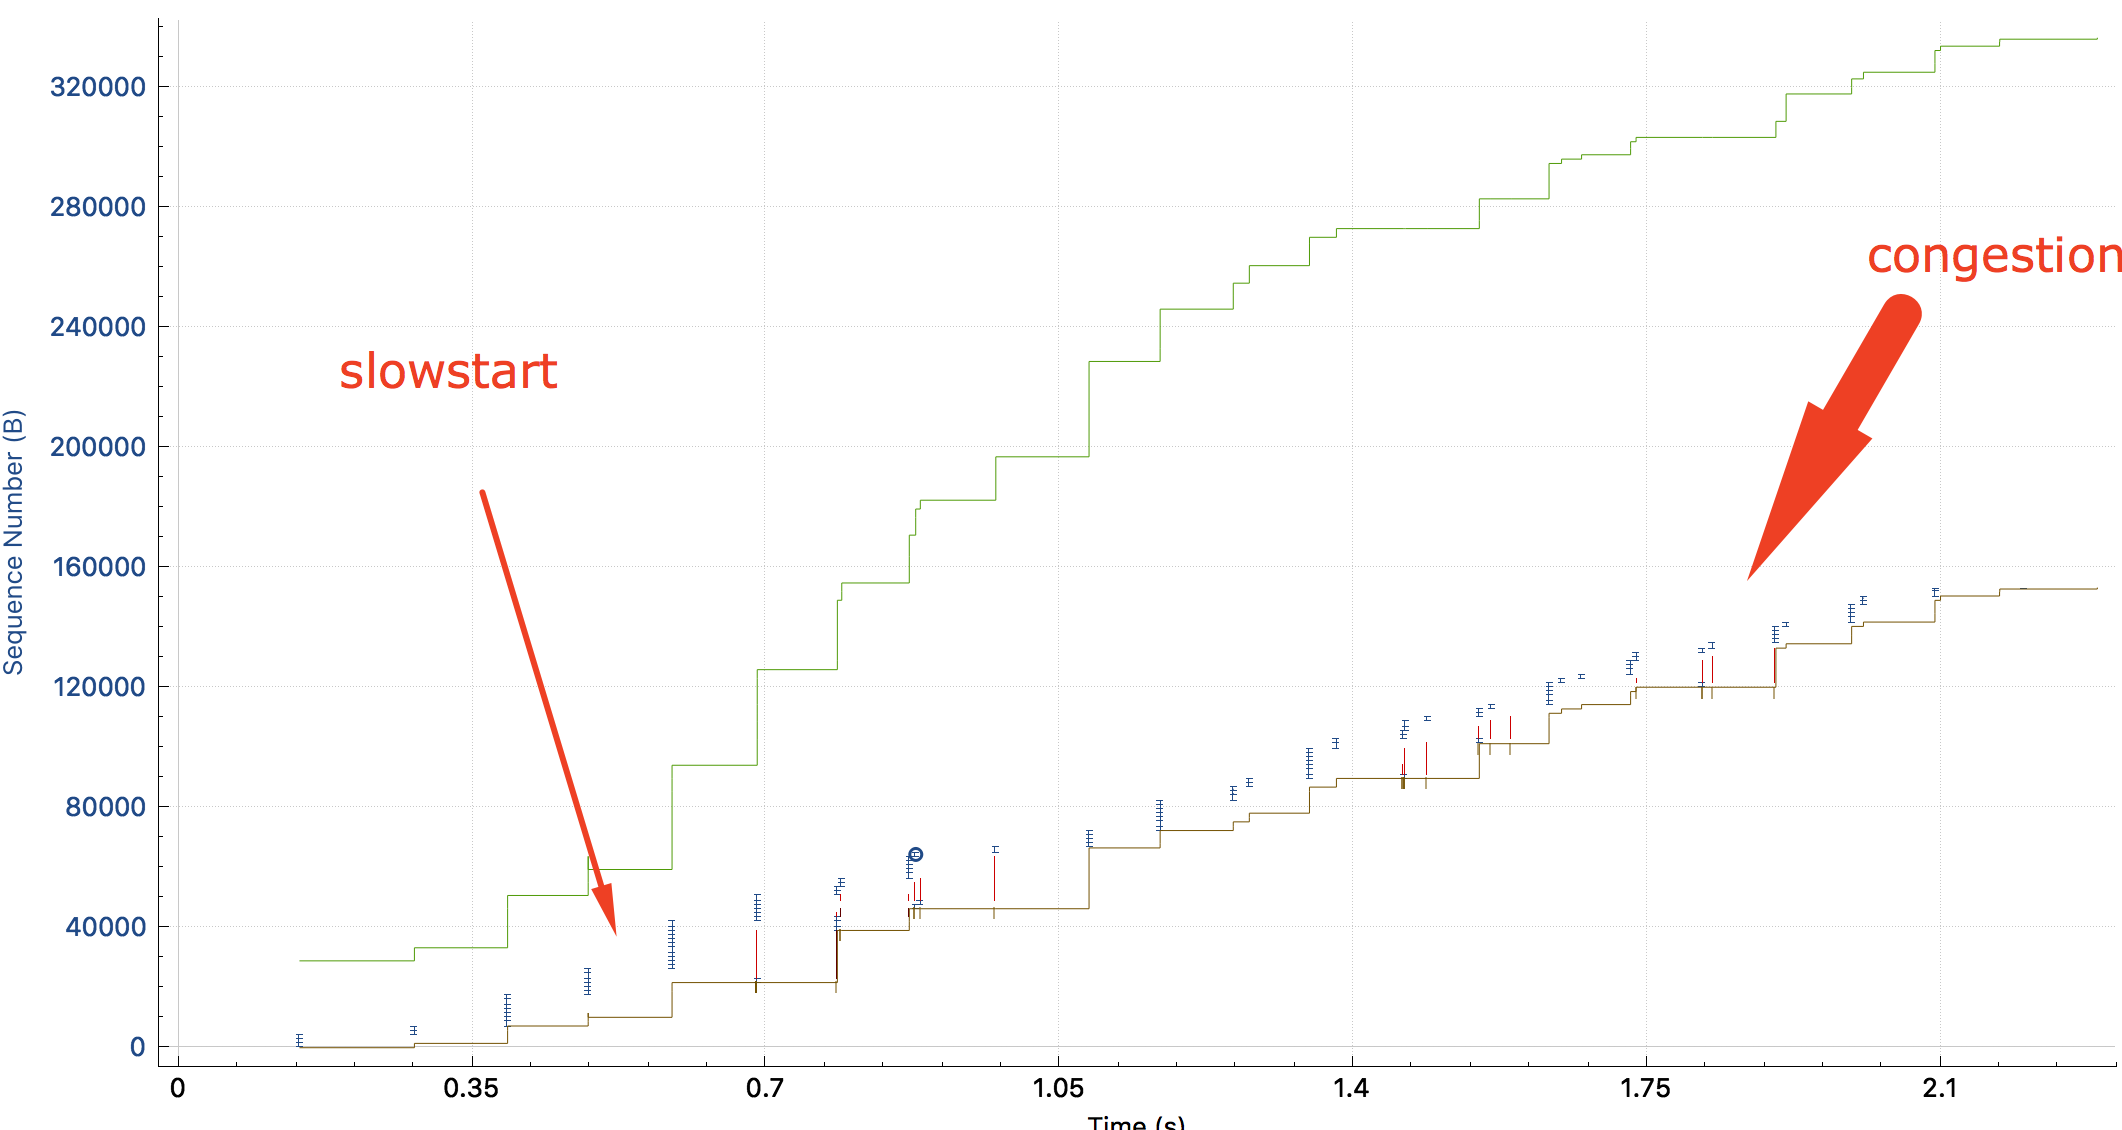
\includegraphics[scale=0.3]{TCPCONGEST.png}
        \end{itemize}

    \end{enumerate}

\end{document}
